\title{INTD262: Aztec Species Classification in Mesoamerica, Linnaean Classification, and Modern Phylogenetics}
\author{Dr. Jordan Hanson - Whittier College Dept. of Physics and Astronomy}
\date{\today}
\documentclass[12pt]{article}
\usepackage[margin=1.5cm]{geometry}
\usepackage{hyperref}
\usepackage{graphicx}
\usepackage{amsmath}
\begin{document}
\maketitle

\section{Introduction}

In this activity, we will compare the Linnaean and modern species classification with the Aztec/Nahua terminology from Chapter 1 of \textit{Science in Latin America}.  First, we will review the Linnaean classifcation system of species.  Second, we will review a modern scientific publication \cite{10.1016/j.cub.2014.03.016} that covers the phylogenetics of hummingbirds.  Third, we will review the Aztec/Nahua terminology for hummingbirds.  Finally, we will compare these results in a temporal and qualitative sense.

\section{Linnaean Classification}

Taxonomy is the identification, naming, and classification of organisms.  Taxonomy emphasizes common physical characteristics of a \textit{taxonomic group}.  The Linnaean classification system developed in the 1700s by Carolus Linnaeus is the foundation for modern taxonomy. Linnaean classification assigns Latin names to a hierarchy of levels, each becoming more specific, and ending with one species.  Linnaeus first published Systema Naturae in the Netherlands (1735).  The 10th edition (1758) classified 4,400 species of animals and 7,700 species of plants. People from around the world sent specimens to be included \footnote{Linnaeus needed a new invention to organize the 12th edition: the index card.}.

A phenotype is the complex set of observable traits of an organism.  If two species have many observable traits in common, we might assign them a similar \textit{taxonomic rank.}  Consider Fig. \ref{fig:1}, in which the taxonomic rank of the red fox is shown.  The levels near the top are the broadest categories, while those near the bottom are the most narrow classifications.  Each level is given a name in Latin.  \textit{Eukarya}, for example, corresponds to all eukaryotic organisms, with cells including a nucleus with DNA.  \textit{Canidae} is the family of wolves, foxes, domestic dogs, wild dogs, coyotes, and jackals.  The \textit{canidae} family has many traits in common.  Make a list below of traits that link this family together.

\begin{figure}[hb]
\centering
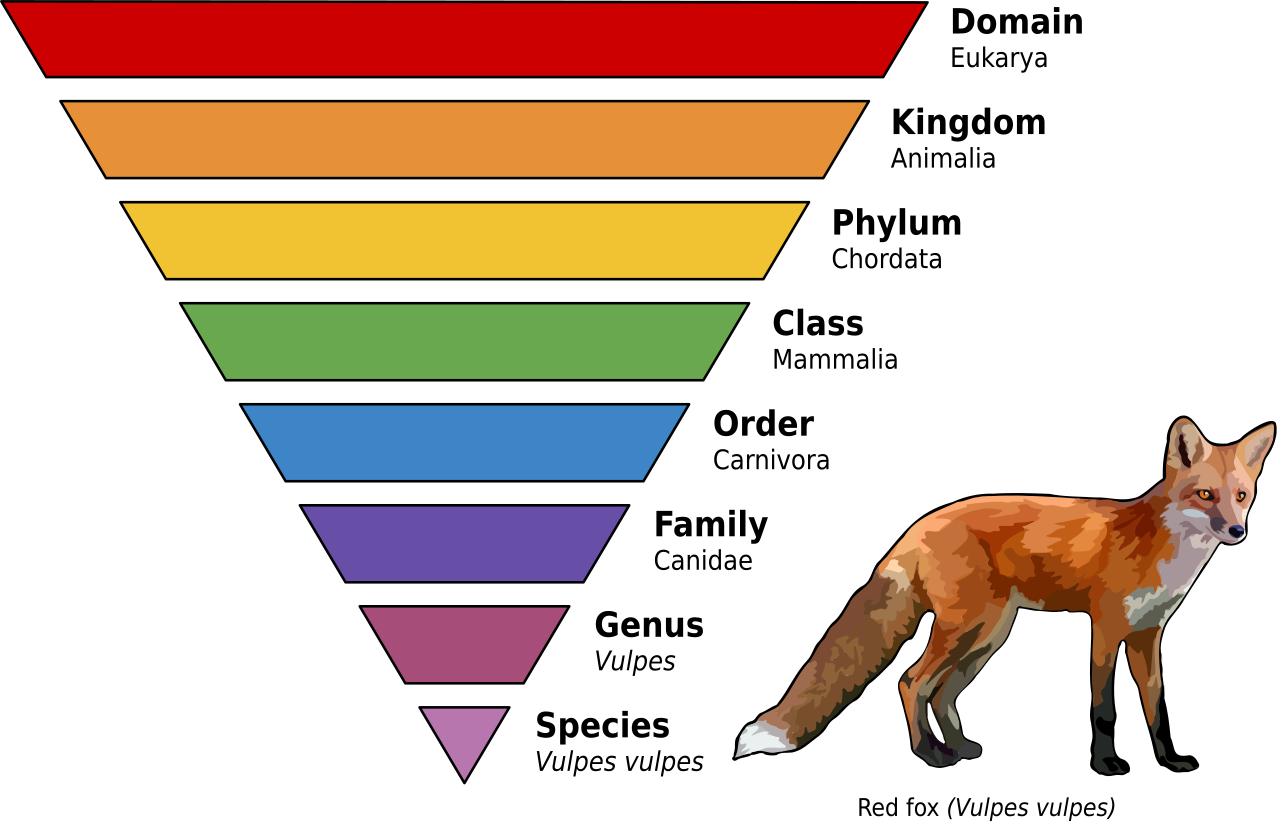
\includegraphics[width=0.35\textwidth]{figures/fox.png}
\caption{\label{fig:1} Taxonomic rank of the red fox.  (Credit: Wikipedia).}
\end{figure}

\vspace{1cm}

\begin{enumerate}
\item List as many traits as you can that are common to all canines: \\ \vspace{2cm}
\item (a) What traits distinguish the red fox (and other foxes) from other canines?  (b) How would you derive a complete classification of the foxes within Canidae? (c) What do you find are the limitations of phenotypic classification in the Linnaean system? \\ \vspace{2cm}
\end{enumerate}

Within the Linnaean system, we refer to a species with the Latin singular nouns associated with the most specific taxonomic levels.  For example, the arctic wolf is called \textit{Canis lupus arctos.}  This tells us we are dealing with a species in the Canidae family, from the genus lupus (wolves), of the artic variety.  The artic variety will have traits that serve as evolutionary adaptations for cold, artic environments with long winters.

Consider species within the order \textit{Apodiformes}, meaning, ``unfooted birds.''  There are three families in this order: \textit{Trochilidae} (hummingbirds), \textit{Hemiprocnidae} (tree swifts), and \textit{Apodidae} (swifts). The family Trochilidae contains 328 species of hummingbirds. At the family level, Trochilidae is divided into two sub-families: Phaethornithinae (hermits) composed of 34 species and a larger group, Trochilinae (trochilines or ``typical'' hummingbirds), with 294 species.

\section{Modern Phylogenetics}

In a recent publication \cite{10.1016/j.cub.2014.03.016}, this taxonomy was updated using modern computational and statistical techniques to estimate the phylogenetics of hummingbird species.  Whittier College has access to the original article and it is posted on Moodle.  The analysis finds 9 \textit{clades}: \textit{Emeralds, Bees, Mountain Gems, Patagona, Coquettes, Brilliants, Magnoes, Hermits, and Topazes.}  Read through the article, and answer the questions below about the findings.

\begin{enumerate}
\item When did hummingbirds differentiate from other birds from a common ancestor? \\ \vspace{1cm}
\item Although there is a great deal of technical jargon in this peer-reviwed research article, what are some key scientific conclusions made by the authors? \\ \vspace{2cm}
\item Which clades are common in the Andes mountain range?  Is the typical range of these species higher or lower than non-Andean species? Quote some specific numbers, if possible.  \\ \vspace{1cm}
\item Have hummingbird-like species ever existed in Europe or Asia? \\ \vspace{1cm}
\end{enumerate}

\section{Aztec Terminology}

In Chapter 1 of \textit{Science in Latin America}, we find an biological account from Father Bernardino Sahag\'{u}n, a Spanish priest who translated indigenous descriptions of Latin American fauna from Nahuatl to 16th-Century Spanish.  In \textit{Historia General de Las Cosas de Nueva Espa\~{n}a}, the Nahuatl-speaking people provide the following zoological nomenclature for hummingbirds, or \textit{huitzitzilin:}

\begin{itemize}
\item \textit{quetzal huitzilin} - colored throats, with bright red elbows on their wings, a green chest and their wings and tail look like fine \textit{quetzals}
\item \textit{xi huitzilin} - all blue, like resplendent turquoise
\item \textit{chalchi huitzilin} - light green like plants
\item \textit{yiauhtic huitzilin} - purple
\item \textit{tlapal huitzilin} - colored and mixed with black
\item \textit{aiopal huitzilin} - light purple
\item \textit{tle huitzilin} - resplendent like hot coals
\item \textit{quapa huitzilin} - tawny yellow
\end{itemize}

Do you see elements of the Linnaean system within these descriptions?  Each species is given a complex name, differentiating the individual species from each other, while at the same time binding them into a family of similar creatures.

\begin{enumerate}
\item Based on these descriptions, make the case for any matches between the Aztec hummingbird families and the clades found in the modern research. As a helpful resource, use a web browser to pull up the Nahuatl dictionary from Wire Humanities: \url{https://nahuatl.wired-humanities.org/}.  From there, you can search the term huitzilin.  \\ \vspace{2.5cm}
\item Use a web browser to pull up a picture of a \textit{quetzal}.  Quetzals are tropical birds from a different family than hummingbirds.  Do a little more searching to identify which hummingbird group most closely resembles quetzals.  Is this finding corroborated by the Nahuatl description? \\ \vspace{2.5cm}
\end{enumerate}

\section{Conclusion}

The goal of this activity is to develop connections between Mesoamerican, Enlightenment period, and modern attempts to understand scientifically the origin of the diversity of species.  This understanding is built upon observation of species characteristics and behavior, and is later quantified with genetic evidence and computational biology.  This activity and our course reading demonstrates that the people of Mesoamerica were classifying species by the 16th century.  Scientists like Carolus Linnaeus began systematizing this knowledge by the 18th century.  One century later, the discovery of DNA occurred.

\begin{figure}
\centering
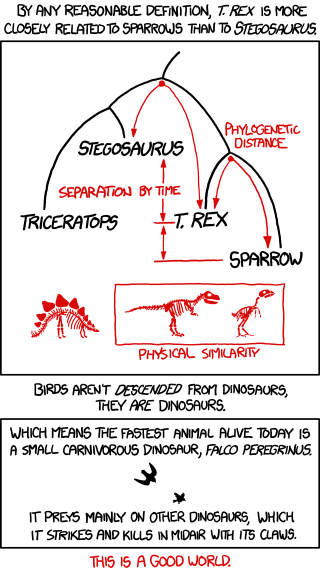
\includegraphics[width=0.3\textwidth]{figures/birds_and_dinosaurs.png}
\caption{\label{fig:3} Phylogenetic distance quantifies the evolutionary relationship between species ... \textit{even dinosaurs!} (Credit: \url{xkcd.com}).}
\end{figure}

\bibliographystyle{plain}
\bibliography{biblio_1}

\end{document}
